\chapter{Calculus in Computer Science}
\label{sec:CS calc}
\epigraph{Machines take me by surprise with great frequency. }{\textit{Alan Turing}}

In most of this module we have focussed on the mathematics, and even when trying to motivate the connection to computer science we have been fairly sketchy. In this chapter we are going to rectify that and discuss some concrete examples of where the material that you have studied here is of relevance to Computer Science, AI, and Machine Learning.\\

If you try to read this chapter before covering all of the basics you may find the examples hard to follow, but if you have finished everything up to \cref{sec:integration}, then you should be fine.\\

This chapter is split into sections, at least one of which should be relevant to each of the degree schemes that this module is included on, \textbf{Computer Science, Computer Science and AI, and Robotics and AI}. This does not mean that you will not find examples of interest in other sections, it just means that I am trying to group the examples thematically.  As with several other chapters, this is a work in progress and will be adapted and expanded over time. Be sure to check back frequently if you want to see the most up to date examples.

\section{LLMs and AI}

Large language models (LLMs) are basically\footnote{This is a real simplification. 3Blue1Brown has a playlist on Neural Networks, available \href{https://www.youtube.com/playlist?list=PLZHQObOWTQDNU6R1_67000Dx_ZCJB-3pi}{here}, which explains more about the applications of calculus to LLMs and what is really going on.} big functions and compositions of functions. Think of it like \cref{fig: simple llm}, where we have input data $x$ which the function sends to an output $f(x)$.\\ 

\begin{figure}[ht]
    \centering
\ThisAltText{A schematic of a LLM as a function.}

    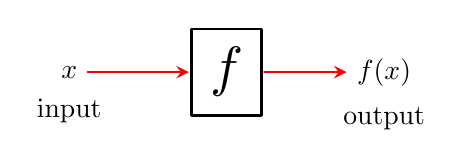
\begin{tikzpicture}[line width=1pt,line cap=round,line join=round, smooth,variable=\x]
  \node[label={below:{input}}] (A) at (0,0) {$x$}; 
 \node[draw,scale=2]        (B) at (2,0) {$f$};
    \node[label={below:{output}}] (C) at (4,0) {$f(x)$}; 

    \draw[red, -stealth] (A) -- (B);  
    \draw[red, -stealth] (B) -- (C);  
    \end{tikzpicture}

    \caption{A schematic of a LLM as a function where the parameters are tuned to take an input and return a specific output.}
        \label{fig: simple llm}
\end{figure}

Here we focus on the simplest case where there is one input, one output, and the function $f$ has a single parameter. In a real system this will be much more complicated, but then you need to be able to use calculus in several variables which is beyond this module. If you are interested in knowing more about the general story let me know and I can provide some further resources.\\

In this picture the function $f$ is a model that tells us how the input is mapped to the output. The parameters in the model tell us how this happens.
\begin{ex}
Consider the function which sends $x$ to $f(x)=ax +b$, this has two parameters $a$ and $b$.
\end{ex}

When training a model we use training data where we already know the true output $y$ that we want to get from a given input $x$. To do this we essentially want to find the ``best'' values of $a$ and $b$, or whatever the parameters are, so that our functions output $\hat{y}$ is as close as possible to the true value $y$.\\

If we are sticking to a simple one parameter model then given the input $x$ we get out put $\hat{y}(w)=f(w,x)$, where $f(x)$ will be a function like $f(w,x)=x+w, wx, e^{wx}, \sin(wx), \dots$. For the training data we then measure the difference between $\hat{y}(w)$ and the true output $y$ for the fixed input $x$. \\

This difference between $\hat(y)(w)$ and $y$ is called an error term, it measures how far out our model is from the true answer. For example $y-\hat{y}(w)$ is a linear error term, while $(y-\hat{y}(w))^{2}$ is a quadratic error term. If we treat the error term as a function of the parameter $w$ and find its critical points this will tell us the values of the parameter that minimise or maximise the error, and we want to minimise the error term.\\

This error function is often called the \textbf{loss function}.  Loss functions appear generally in decision theory and the study of optimisation problems. They appear whenever you are training an AI or LLM, where they measure the deviation of the model's output against the true value for the training data. \\

%It could be that you are checking if your model can perform a mathematical calculation, in which case you will be comparing two numbers, the output number against the true solution. It could also be a more general problem where you are training a model to recognise images, in which case you will be comparing the answer output by your model to the true answer. The main idea is that this can always be described by some function. In fact a key step will be deciding what is an appropriate loss function for your problem. \\
%
%Once we have the loss function, training is then the process of tweaking our model to minimise the loss function, so that the output of your model most closely matches the true values.\\

A conventional choice of loss function is the quadratic loss function
\begin{equation}
\lambda(w)=\left(\hat{y}(w)-y\right)^{2}
\label{eq: quadratic loss}
\end{equation}

Again the idea that given a function $f$ with a single free parameter $w$ we want to minimise $\lambda(w)$ for fixed input $x$ and fixed true output $y$. The optimisation method used is called \textbf{gradient flow}. In a one dimensional case we are solving 
\begin{equation*}
\frac{\ud \lambda}{\ud w}=0
\end{equation*}
for $w$, to get the optimal $\hat{y}(w)$ for a given $x$.

\begin{app}
Consider the one parameter model $\hat{y}(w)=\sin(wx)$ and the quadratic loss function in \cref{eq: quadratic loss}. If the input is $x=\pi$ and the desired output is $y=0$ then the loss function becomes
\begin{equation*}
\lambda(w)=\left(\sin(w\pi)-0\right)^{2}=\left(\sin(w\pi)\right)^{2}.
\end{equation*}
Then 
\begin{align*}
\frac{\ud \lambda}{\ud w}	&=2\pi\sin(w\pi)\cos(w\pi)\\
					&=\pi\sin(2w\pi).
\end{align*}
This is zero when $w=\pm1,\pm2,\pm3, \dots$ or $w=\pm1/2, \pm 3/2, \pm5/2, \dots$. i.e. $w$ is either an integer or a half-integer.

Looking at the second derivative we see that 
\begin{equation*}
\frac{\ud^{2} \lambda}{\ud w^{2}}=2\pi^{2}\cos(2w\pi),
\end{equation*}
and that 
\begin{align*}
\frac{\ud^{2} \lambda}{\ud w^{2}}\left(\pm1,\pm2, \dots\right)&>0\\
\frac{\ud^{2} \lambda}{\ud w^{2}}\left(\pm\frac{1}{2},\pm\frac{3}{2}, \dots\right)&<0
\end{align*}
So integer values of $w$ are minima and half integer values are maxima.\\

For all of these values $f:\pi\mapsto 0$ so you would need to look at more training data to fix a single value of $w$.
\end{app}

It is important to note that while optimisation can get the output closer to the true value, how close it can get depends on how good the choice of model $f$ is. 
\begin{ex}
Consider the model
\begin{equation*}
\hat{y}(w)=\frac{wx}{1+w^{2}x^{2}},
\end{equation*}
alongside the quadratic loss function.  If the target output for input $x=1$ is $y=2$ what is the optimal value of $w$?\\

For $x=1$ and $y=2$ the loss function becomes
\begin{equation*}
\hat{y}(w)=\left(\frac{w}{1+w^{2}}-2\right)^{2}.
\end{equation*}

Note here that $w/(1+w^{2})<1/2$ so we can never get $\lambda(w)=0$, i.e. this model is a bad fit for the training data.\\

If we optimise anyway then we get
\begin{align*}
\frac{\ud \lambda}{\ud w}	&2\left(\frac{w}{1+w^{2}}-2\right)\frac{\ud}{\ud w}\left(\frac{w}{1+w^{2}}\right)\\
					&=2\left(\frac{w}{1+w^{2}}-2\right)\frac{(1-w^{2})}{(1+w^{2})^{2}}.
\end{align*}
We know that the first bracket does not vanish so this is zero when $1-w^{2}=0$ giving $w=\pm1$. If $w=1$ then $\lambda(+1)=9/4$ while $\lambda(-1)=25/4$ so $w=+1$ is the minimum. Bot for this choice of $w$ the output is
\begin{equation*}
\hat{y}(1)=\frac{1}{1+1}=\frac{1}{2}\neq 2
\end{equation*}
So we do not get a match for the desired output.
\end{ex}

This example of optimisation not working is a useful warning as it shows us that while optimisation is a powerful and useful model you still need to start from a sensible model.

\section{Robotics}
\textcolor{red}{To be added.}